\chapter{PHÂN TÍCH VÀ THIẾT KẾ HỆ THỐNG}\label{chap2_intro}
\vspace{-40pt}

\section{Yêu cầu hệ thống}
\subsection{Yêu cầu chức năng}
\begin{itemize}
    \item \textbf{UC01 -- Đăng ký:} Người dùng chưa đăng nhập có thể tạo tài khoản mới; hệ thống kiểm tra tính đầy đủ, hợp lệ của thông tin trước khi lưu.
    \item \textbf{UC02 -- Đăng nhập:} Người dùng cung cấp thông tin xác thực; hệ thống kiểm tra thông tin đăng nhập và trạng thái tài khoản trước khi cho phép truy cập.
    \item \textbf{UC03 -- Xem, tìm kiếm và lọc sản phẩm:} Người dùng có thể xem sản phẩm, tìm kiếm theo từ khóa, lọc theo danh mục, khoảng giá hoặc thương hiệu và xem thông tin chi tiết.
    \item \textbf{UC04 -- Quản lý giỏ hàng:} Khách hàng có thể thêm sản phẩm vào giỏ hàng, thay đổi số lượng hoặc xóa sản phẩm; giỏ hàng được quản lý theo tài khoản.
    \item \textbf{UC05 -- Đặt hàng:} Khách hàng tạo đơn từ giỏ hàng, chọn địa chỉ nhận hàng, có thể áp dụng voucher và chọn phương thức thanh toán; hệ thống kiểm tra thông tin, ưu đãi và tồn kho trước khi tạo đơn.
    \item \textbf{UC06 -- Thanh toán:} Khách hàng thanh toán khi nhận hàng hoặc trực tuyến; với giao dịch trực tuyến, hệ thống gửi yêu cầu đến cổng thanh toán và cập nhật trạng thái theo kết quả.
    \item \textbf{UC07 -- Theo dõi và hủy đơn hàng:} Khách hàng xem đơn hàng, theo dõi trạng thái xử lý và thanh toán, đồng thời gửi yêu cầu hủy khi đơn còn ở trạng thái cho phép.
    \item \textbf{UC08 -- Quản lý tài khoản:} Khách hàng xem và cập nhật thông tin cá nhân, thông tin liên hệ, mật khẩu và sổ địa chỉ giao hàng.
    \item \textbf{UC09 -- Quản lý đơn hàng:} Nhân viên và quản trị viên xem, kiểm tra và xử lý đơn hàng theo quyền được cấp, từ xác nhận đơn đến cập nhật trạng thái xử lý.
    \item \textbf{UC10 -- Kiểm tra tồn kho:} Nhân viên tra cứu số lượng tồn kho của sản phẩm; chức năng này chỉ phục vụ xem thông tin, không điều chỉnh số lượng.
    \item \textbf{UC11 -- Quản lý sản phẩm:} Quản trị viên thêm, chỉnh sửa và cập nhật trạng thái sản phẩm, bao gồm thông tin mô tả, giá niêm yết, phân loại và thông số kỹ thuật.
    \item \textbf{UC12 -- Quản lý danh mục:} Quản trị viên thêm, chỉnh sửa hoặc cập nhật trạng thái danh mục sản phẩm.
    \item \textbf{UC13 -- Quản lý người dùng:} Quản trị viên tìm kiếm và quản lý tài khoản; có thể thêm hoặc cập nhật tài khoản nhân viên, cũng như xem và thay đổi trạng thái tài khoản khách hàng.
    \item \textbf{UC14 -- Quản lý kho:} Quản trị viên theo dõi tồn kho và nhập hoặc điều chỉnh số lượng sản phẩm; hệ thống kiểm tra dữ liệu để số lượng không nhỏ hơn 0.
    \item \textbf{UC15 -- Xem thống kê:} Quản trị viên xem số liệu về doanh thu, đơn hàng và tình hình sản phẩm theo khoảng thời gian được chọn.
    \item \textbf{UC16 -- Quản lý chương trình giảm giá:} Quản trị viên tạo, chỉnh sửa, kích hoạt hoặc kết thúc chương trình giảm giá, áp dụng cho toàn trang hoặc sản phẩm được chọn với mức giảm theo phần trăm hoặc số tiền.
    \item \textbf{UC17 -- Quản lý voucher:} Quản trị viên tạo và quản lý voucher, gồm mã, mức giảm, thời hạn, giá trị đơn tối thiểu và các giới hạn sử dụng.
    \item \textbf{UC18 -- Áp dụng voucher khi đặt hàng:} Khách hàng nhập mã voucher khi đặt hàng; hệ thống kiểm tra điều kiện và giới hạn sử dụng, tính lại tổng tiền và ghi nhận lượt sử dụng khi tạo đơn.
\end{itemize}

\subsection{Yêu cầu phi chức năng}
Thông tin đầu vào cần được kiểm tra trước khi xử lý; thao tác thay đổi dữ liệu cần được thực hiện qua các luồng có kiểm soát. Dữ liệu tài khoản và đơn hàng được lưu trong cơ sở dữ liệu MySQL. Giao diện cần trình bày các chức năng rõ ràng trên trình duyệt máy tính và có thể sử dụng các tương tác JavaScript hiện có.

\section{Tác nhân và quy trình nghiệp vụ}
\subsection{Tác nhân}
\begin{itemize}
    \item \textbf{Khách vãng lai:} Là người truy cập website nhưng chưa được xác thực đăng nhập vào hệ thống. Khách vãng lai có thể đã có hoặc chưa có tài khoản. Tác nhân này chỉ có quyền đăng ký, đăng nhập, xem, tìm kiếm và lọc sản phẩm. Nếu muốn thực hiện thao tác với giỏ hàng hoặc mua hàng, hệ thống sẽ yêu cầu Khách vãng lai phải đăng nhập để chuyển thành Khách hàng.
    \item \textbf{Khách hàng:} Là người đã có tài khoản và đăng nhập vào hệ thống. Khách hàng có thể xem sản phẩm, quản lý giỏ hàng, đặt hàng, thanh toán, theo dõi và hủy đơn hàng theo điều kiện cho phép, đồng thời quản lý thông tin tài khoản
    \item \textbf{Nhân viên:} Hỗ trợ hoạt động bán hàng và xử lý đơn hàng trong phạm vi quyền được cấp và chỉ có thể kiểm trasố lượng tồn kho của sản phẩm.
    \item \textbf{Quản trị viên:} Là người có quyền quản lý và vận hành hệ thống. Quản trị viên có thể quản lý đơn hàng, sản phẩm, danh mục, người dùng, kho và xem các số liệu thống kê.
    \item \textbf{Cổng thanh toán:} Là hệ thống thanh toán bên ngoài được sử dụng để xử lý các giao dịch thanh toán trực tuyến và trả kết quả giao dịch về cho hệ thống.
    \item \textbf{Google Identity:} Là dịch vụ xác thực của Google cho phép người dùng đăng nhập vào hệ thống bằng tài khoản Google của họ.
\end{itemize}

\subsection{Quy trình đặt hàng}
Khách hàng chọn sản phẩm và số lượng để đưa vào giỏ hàng. Khi tiến hành đặt hàng, hệ thống kiểm tra dữ liệu đơn hàng và các mặt hàng trong giỏ, tạo đơn cùng chi tiết đơn, cập nhật số lượng tồn kho và xóa các dòng giỏ hàng đã đặt. Các thao tác liên quan được xử lý trong giao dịch cơ sở dữ liệu. Đơn hàng trong phạm vi đồ án sử dụng hình thức COD.

\subsection{Quy trình hủy đơn}
Khách hàng gửi yêu cầu hủy đơn từ danh sách đơn hàng. Hệ thống kiểm tra quyền sở hữu và trạng thái đơn trước khi xử lý; nếu đủ điều kiện, thông tin đơn được cập nhật và số lượng hàng được hoàn lại kho.

\section{Thiết kế kiến trúc}
Hệ thống được tổ chức quanh front controller và router. Router chuyển yêu cầu đến controller tương ứng; controller gọi model để thực hiện nghiệp vụ và lấy dữ liệu; view nhận dữ liệu để hiển thị trang. Các model kết nối MySQL thông qua PDO. Cấu trúc này giữ phần giao diện tách biệt tương đối với xử lý nghiệp vụ và truy vấn dữ liệu.

\section{Thiết kế cơ sở dữ liệu}
Cơ sở dữ liệu lưu trữ các nhóm thông tin chính: người dùng và tài khoản; danh mục và sản phẩm; giỏ hàng và chi tiết giỏ hàng; đơn hàng và chi tiết đơn hàng; lịch sử kho. Các bảng được liên kết bằng khóa chính, khóa ngoại và các ràng buộc phù hợp với quan hệ nghiệp vụ. Bảng giao dịch thanh toán có trong schema nhưng chưa được sử dụng trong luồng đặt hàng hiện tại.

\section{Công cụ và môi trường}
Ứng dụng được xây dựng bằng PHP, MySQL, HTML, CSS và JavaScript; PDO được dùng để kết nối cơ sở dữ liệu. Môi trường triển khai của dự án sử dụng máy chủ web Apache trong bộ XAMPP.

\section{Sơ đồ Use Case tổng quan}
\begin{figure}[H]
    \centering
    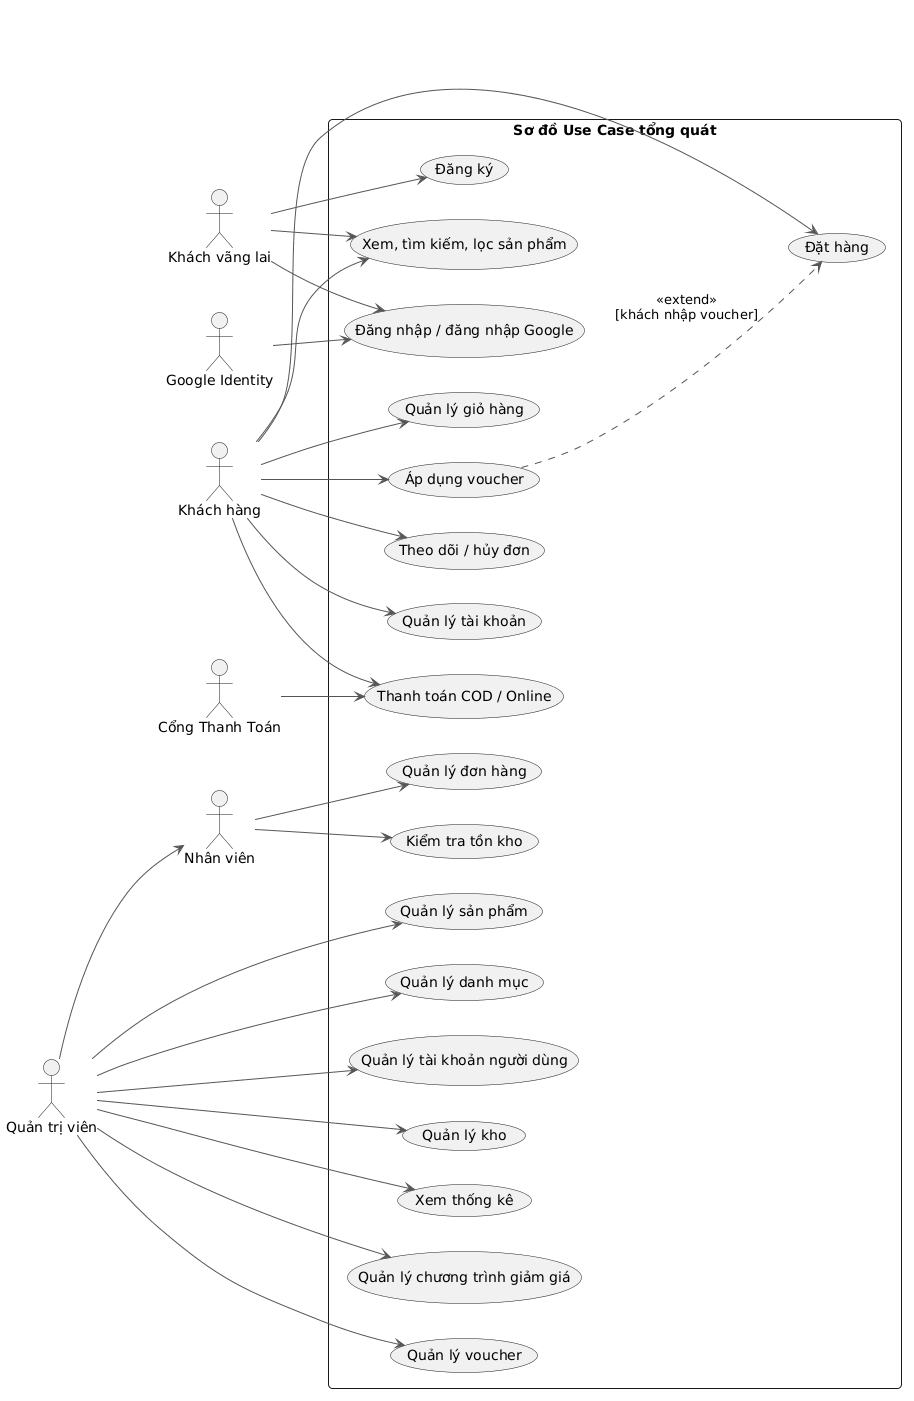
\includegraphics[width=0.72\textwidth, keepaspectratio]{Chapter_2/Images_c2/So_do_UC_tong_quan.png}
    \caption{Sơ đồ Use Case tổng quát của hệ thống website T\&T Computer}
    \label{fig:use-case-tong-quan}
\end{figure}

\section{Sơ đồ cơ sở dữ liệu:}
\begin{figure}[H]
    \centering
    \includegraphics[width=0.9\textwidth, keepaspectratio]{Chapter_2/images_c2/db.png}
    \caption{Sơ đồ cơ sở dữ liệu}
    \label{fig:db-diagram}
\end{figure}

\section{Sơ đồ lớp:}
\begin{figure}[H]
    \centering
    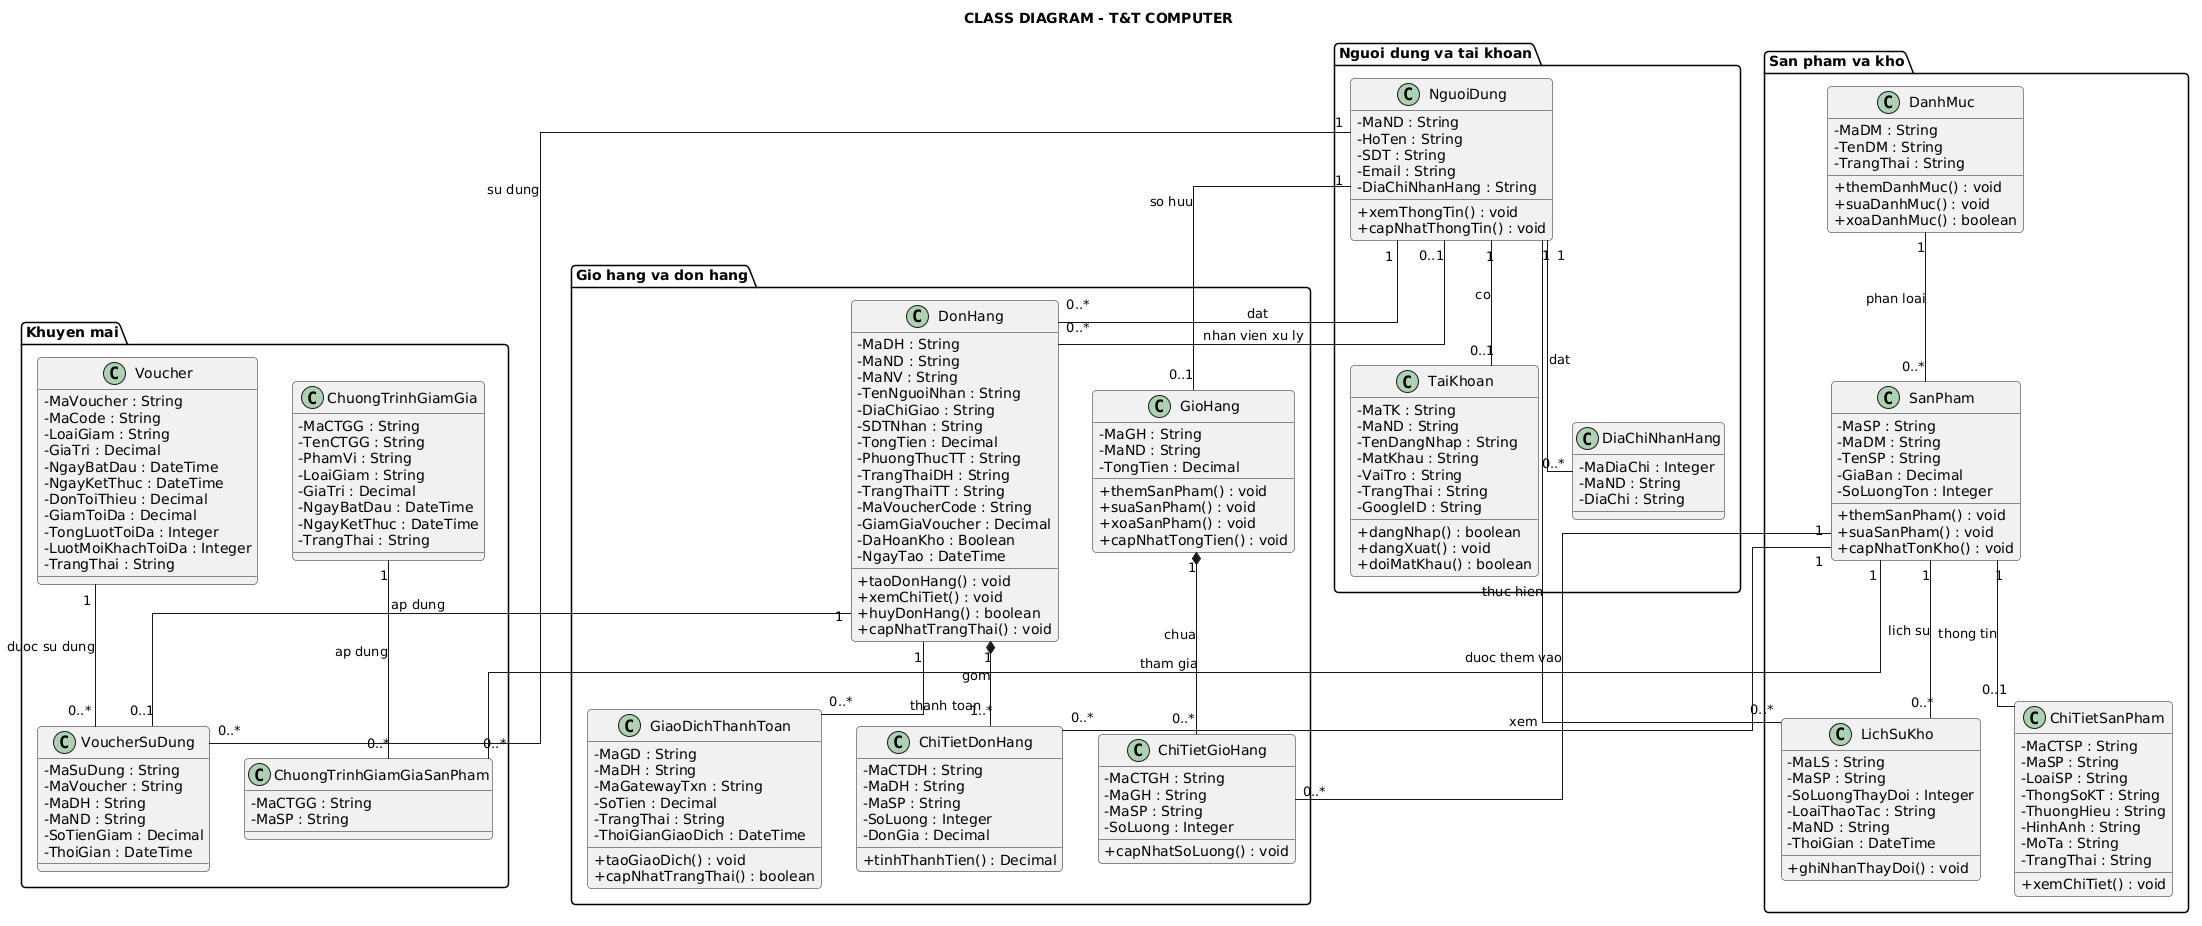
\includegraphics[width=0.9\textwidth, keepaspectratio]{Chapter_4/image/Sơ đồ class.png}
    \caption{Sơ đồ lớp}
    \label{fig:class-diagram}
\end{figure}
